\documentclass[10pt,pdf,hyperref={unicode}]{beamer}

\usepackage[normalem]{ulem}
\usepackage{qrcode}
\usepackage{array}
\usepackage[T2A]{fontenc}
\usepackage[utf8]{inputenc}
\usepackage{colortbl}
\usepackage{listings}

\setbeamertemplate{navigation symbols}{}

\usetheme{default}

\usepackage{array}
\newcolumntype{L}[1]{>{\raggedright\let\newline\\\arraybackslash\hspace{0pt}}m{#1}}
\newcolumntype{C}[1]{>{\centering\let\newline\\\arraybackslash\hspace{0pt}}m{#1}}
\newcolumntype{R}[1]{>{\raggedleft\let\newline\\\arraybackslash\hspace{0pt}}m{#1}}

\title{Семинар 8: Intel x86 assembly}
\date{14 января, 2020}


\begin{document}

\begin{frame}
  \titlepage
\end{frame}

\begin{frame}{Ассемблер}
    \begin{itemize}
        \item Процессор выполняет \emph{инструкции}
        \item Выполнение инструкций — комплексный процесс
        \item Стадии выполнения: fetch, decode, execute, memory access, writeback
        \item Современные процессоры — \emph{суперскалярные}, то есть выполняют несколько стадий одновременно
        \item Dynamic execution
    \end{itemize}
\end{frame}

\begin{frame}{Pipelining}
\center\begin{figure}[!]
    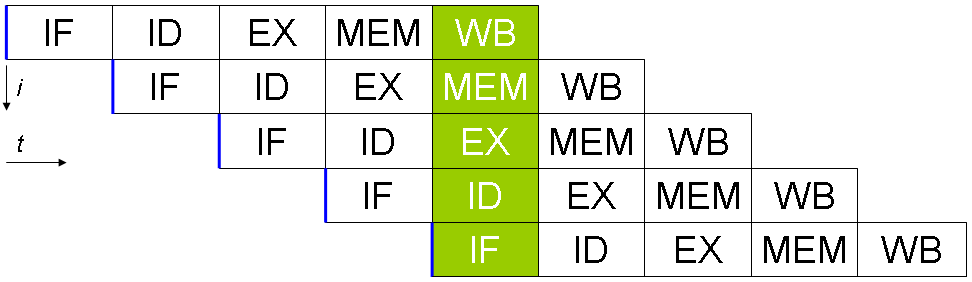
\includegraphics[width=300px]{pipeline.png}
    \caption{Pipeline современных процессоров (из Wikipedia)}
\end{figure}
\end{frame}

\begin{frame}{Ассемблер Intel x86}
    \begin{itemize}
        \item Впервые появился в процессоре Intel 8086
        \item CISC-архитектура
        \item Два синтаксиса: Intel syntax, AT\&T syntax
    \end{itemize}
\end{frame}


\begin{frame}{Регистры}
\begin{itemize}
    \item Регистры — очень быстрая, но маленькая память
    \item Под x86 — \textbf{32 бита}, под x86-64 — \textbf{64 бита}
    \item 32-bit registers: \textbf{eax}, \textbf{ebx}, \textbf{ecx}, \textbf{edx}, \textbf{esi}, \textbf{edi}
    \item 64-bit registers: \textbf{rax}, \textbf{rbx}, \textbf{rcx}, \textbf{rdx}, \textbf{rsi}, \textbf{rdi}, \textbf{r8}-\textbf{r15}
    \item Хранят числа в two's complement little endian представлении
\end{itemize}
\end{frame}

\begin{frame}{Вложенность регистров}
\begin{center}
\begin{tabular}{ |C{0.75cm}|C{0.75cm}|C{0.75cm}|C{0.75cm}|C{0.75cm}|C{0.75cm}|C{0.75cm}|C{0.75cm}| }
    \hline
    7 & 6 & 5 & 4 & 3 & 2 & 1 & 0 \\
    \hline
    \multicolumn{8}{|c|}{\textbf{rax}}\\
    \hline
    \multicolumn{4}{|c|}{} & \multicolumn{4}{c|}{\textbf{eax}}\\
    \hline
    \multicolumn{6}{|c|}{} & \multicolumn{2}{c|}{\textbf{ax}}\\
    \hline
    \multicolumn{6}{|c|}{} & \textbf{ah} & \textbf{al}\\
    \hline
\end{tabular}
\end{center}
\end{frame}

\begin{frame}{Инструкции}
\begin{itemize}
    \item Кодируются различным количеством байт: от 1 до 6
    \item При decode транслируются в более низкоуровневый $\mu$-op
    \item Запись: \lstinline{LABEL: INST ARGS}
    \item В основном все инструкции — бинарные
    \item Аргументом могут выступать либо регистр, либо память, либо \emph{immediate value}
    \item По крайней мере один регистр должен быть среди аргументов!
\end{itemize}
\end{frame}


\begin{frame}{Примеры инструкций}
\begin{itemize}
    \item \lstinline{add rax, rbx}
    \item \lstinline{cmp rax, rbx}
    \item \lstinline{inc r8}
\end{itemize}
\end{frame}


\begin{frame}{Различия синтаксисов}
\begin{itemize}
    \item Intel: \lstinline{INST DST, SRC}
    \item AT\&T: \lstinline{INST SRC, DST}
\end{itemize}
\end{frame}


\begin{frame}{EFLAGS}
\begin{itemize}
    \item Специальный регистр, который хранит \emph{флаги}
    \item Каждому флагу соответствует определённый бит в EFLAGS
    \item Флаги выставляются в результате выполнения арифметических инструкций
\end{itemize}
\end{frame}


\begin{frame}{Примеры флагов}
\begin{itemize}
    \item \textbf{ZF} выставляется, если был получен 0
    \item \textbf{SF} выставляется, если было получено отрицательное число
    \item \textbf{СF} выставляется при возникновении переноса в MSB (carry flag)
    \item \textbf{СF} выставляется при возникновении знакового переполнения (overflow flag)
\end{itemize}
\end{frame}

\begin{frame}{Контроль за выполением программы}
\begin{itemize}
    \item Процессор позволяет <<прыгать>> в любую точку программы
    \item Такие прыжки делятся на три класса: безусловные, условные и вызовы процедур
    \item Безусловные просто меняют текущий IP на заданный
    \item Условные меняют текущий IP на заданный, если в EFLAGS есть определённый флаг
    \iteme Вызовы процедур специальным образом подготавливают окружение для вызова функций
\end{itemize}
\end{frame}


\begin{frame}
\center\Huge{Grazie!}
\end{frame}


\end{document}
